\documentclass[12pt,a4paper]{article}
\usepackage[UTF8]{ctex}
\usepackage{graphicx}
\usepackage{geometry}
\usepackage{ulem}
\usepackage{enumitem}
\usepackage{titlesec}
\usepackage{multicol}
\usepackage[export]{adjustbox}
\usepackage{amsmath}  % 推荐用于更好的数学排版
\usepackage[utf8]{inputenc}
\usepackage{CJKutf8}
\usepackage{fancyhdr}
\usepackage{lastpage}
\usepackage{tabularx}
\usepackage{lastpage}
\usepackage{float}
\usepackage{caption}
\usepackage{subcaption}
% 页眉页脚设置
\pagestyle{fancy}
\fancyhf{} % 清除所有页眉页脚
% 设置页眉内容
%-==========1. 填写从第二页开始 每页第一行的信息==========-
\fancyhead[C]{
    \makebox[4.5em][c]{实验名称：} \uline{\makebox[14em][c]{OrCAD软件使用练习}} 
    \makebox[2.5em][c]{姓名：} \uline{\makebox[4em][c]{}} 
    \makebox[2.5em][c]{学号：} \uline{\makebox[5em][c]{}}
}%--------------------------------------------------------
\fancyfoot[C]{第 \thepage\ 页，共 \pageref{LastPage} 页}

% 取消页眉和页脚的下划线
\renewcommand{\headrulewidth}{0pt} % 页眉横线粗细设为0
\renewcommand{\footrulewidth}{0pt} % 页脚横线粗细设为0

% 调整页眉高度
\setlength{\headheight}{50pt}

% 设置plain样式（用于第一页）
\fancypagestyle{plain}{
    \fancyhf{} % 清除所有页眉页脚
    \renewcommand{\headrulewidth}{0pt} % 隐藏页眉横线
    \fancyfoot[C]{第 \thepage\ 页，共 \pageref{LastPage} 页}
}
% 设置页面边距
\geometry{left=2.54cm,right=1.5cm,top=2.54cm,bottom=2.54cm}

% 设置正文字体大小为小四
\renewcommand{\normalsize}{\fontsize{12pt}{18pt}\selectfont}
% 设置章节格式
\titleformat{\section}{\fontsize{16pt}{24pt}\selectfont\bfseries}{\thesection}{1em}{} % 一级标题：三号
\titleformat{\subsection}{\fontsize{15pt}{22.5pt}\selectfont\bfseries}{\thesubsection}{1em}{} % 二级标题：小三

\begin{document}
\thispagestyle{plain}%第一页使用 plain 样式，而不是默认的 fancy 样式，第一页不再显示页眉
% 标题 标题部分 - 两栏布局
\begin{multicols}{2}
    % 左栏：图片和实验报告标题
    % 左栏：使用空行创建前三行
    \noindent
    ~\\ % 第一行
    ~\\ % 第二行
    ~\\ % 第三行
    \hphantom{占位}% 使用空占位符
    \raisebox{-0.5\baselineskip}% 图片向下移动半行
    {
\includegraphics[width=1.85in,height=0.58in]{figure/ZJU.jpg}}
    \hspace{.5em}% 图片和标题之间的间距
    \raisebox{0pt}[\height][0pt]% 标题底部对齐
    {\textbf{\fontsize{26pt}{30pt}\selectfont 实验报告}}
    
    \columnbreak % 换到右栏
    
    % 右栏：个人信息
    % 右栏：个人信息 - 靠右对齐 
%-==========2. 填写个人信息==========-
    \begin{flushright}
        \makebox[3em][l]{专业：} \uline{\makebox[9em][c]{}} \\
        \makebox[3em][l]{姓名：} \uline{\makebox[9em][c]{}} \\
        \makebox[3em][l]{学号：} \uline{\makebox[9em][c]{}} \\
        \makebox[3em][l]{日期：} \uline{\makebox[9em][c]{2025年11月25日}} \\
        \makebox[3em][l]{地点：} \uline{\makebox[9em][c]{紫金港东四216}} \\
    \end{flushright}
   
\end{multicols}
% 课程名称等信息（单栏）
%-==========3. 填写课程信息==========-
\noindent\small
课程名称： \uline{电子电路设计实验I} \hfill 指导老师： \uline{施红军、叶险峰、邓靖靖} \hfill 成绩： \uline{\hspace{3cm}} \\
实验名称： \uline{OrCAD软件使用练习} \hfill 实验类型： \uline{验证类实验} \hfill 同组学生姓名： \uline{}
%-==========4. 正文开始==========-
\section*{一、实验目的}

1．了解OrCAD套件中的Capture和PSpice A/D软件的常用菜单和命令的使用。 

2．掌握OrCAD中Capture软件的电路图输入和编辑方法。 

3．学习OrCAD中PSpice A/D软件的分析设置、仿真、波形查看的方法。 

4．学习半导体器件特性、电路特性的仿真分析方法。 
\section*{二、实验任务与要求}
1.二极管特性仿真

2.桥式整流电路瞬态分析

3.稳压二极管电路瞬态分析


\section*{三、实验步骤、调试过程、实验数据记录}
\subsection*{3.1 二极管特性仿真}

(1)输入电路图

取元件VSRC、R、D1N4148、AGND，按图\ref{fig:1.1}所示连接成电路图.电阻阻值设为1kΩ，
电压源VSRC名称设为$V_s$

\begin{figure}[H]
    \centering
    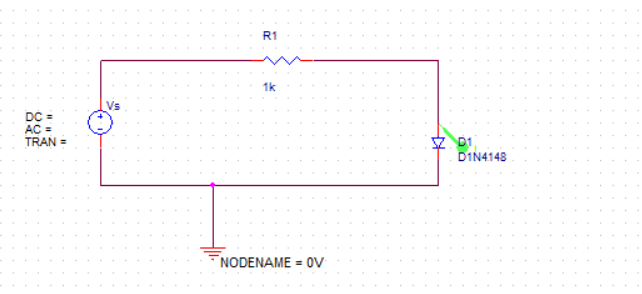
\includegraphics[width=0.45\textwidth]{figure/diode_circuit.png}
    \caption{二极管仿真电路图}
    \label{fig:1.1}
\end{figure}

(2)设置仿真参数

二极管伏安特性的仿真分析对电压源 Vs
进行直流扫描（DC Sweep）分析。为了仿真
二极管的正向导通特性、反向特性和击穿特
性，应使 Vs 的变化范围足够大。所以，二极
管测试电路的直流扫描分析参数可设置为：
扫描变量类型为电压源，扫描变量为 Vs，扫
描类型为线性扫描，初始值为-200V，终值为
40V，增量为 0.1V，如图 \ref{fig:1.2}所示。

\begin{figure}[H]
    \centering
    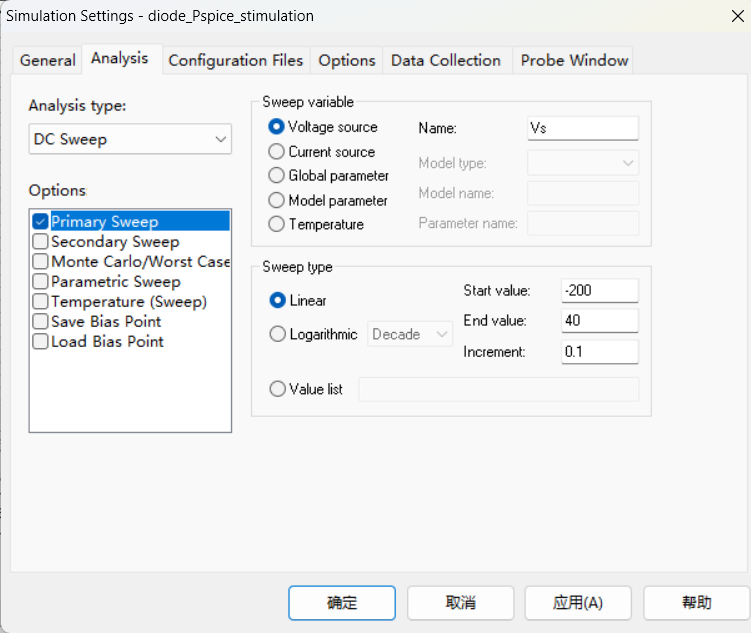
\includegraphics[width=0.55\textwidth]{figure/diode_dcSweep_setting.png}
    \caption{二极管直流分析参数设置图}
    \label{fig:1.2}
\end{figure}

(3)运行仿真，查看二极管伏安特性曲线

起初得到的仿真结果是二极管电流与电压源的关系。设置x轴变量如图\ref{fig:1.3a}所示，选择二极管两端电压作为x轴变量，得到二极管的伏安特性曲线，如图\ref{fig:1.3b}所示。

\begin{figure}[H]
    \centering
    \begin{subfigure}{0.48\textwidth}
        \centering
    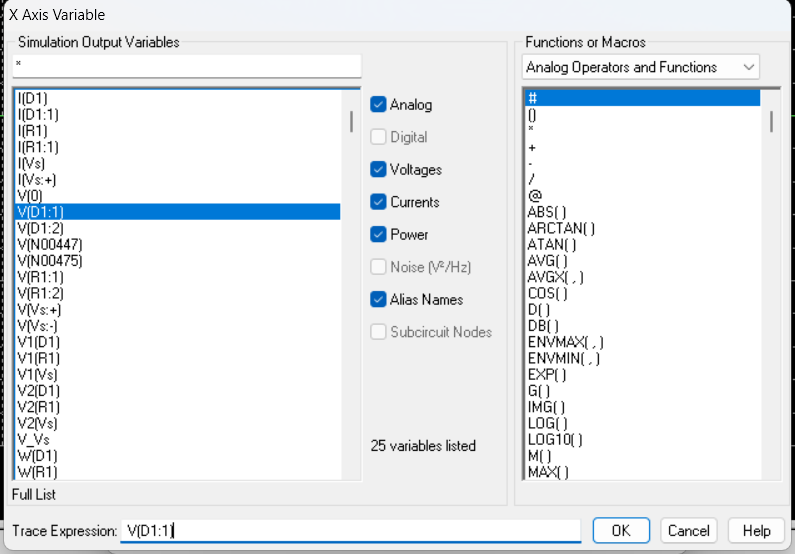
\includegraphics[width=\textwidth]{figure/diode_curve_setting.png}
    \caption{二极管伏安特性曲线坐标轴设置图}
    \label{fig:1.3a}
\end{subfigure}
\hfill
    
\begin{subfigure}{0.49\textwidth}
        \centering
        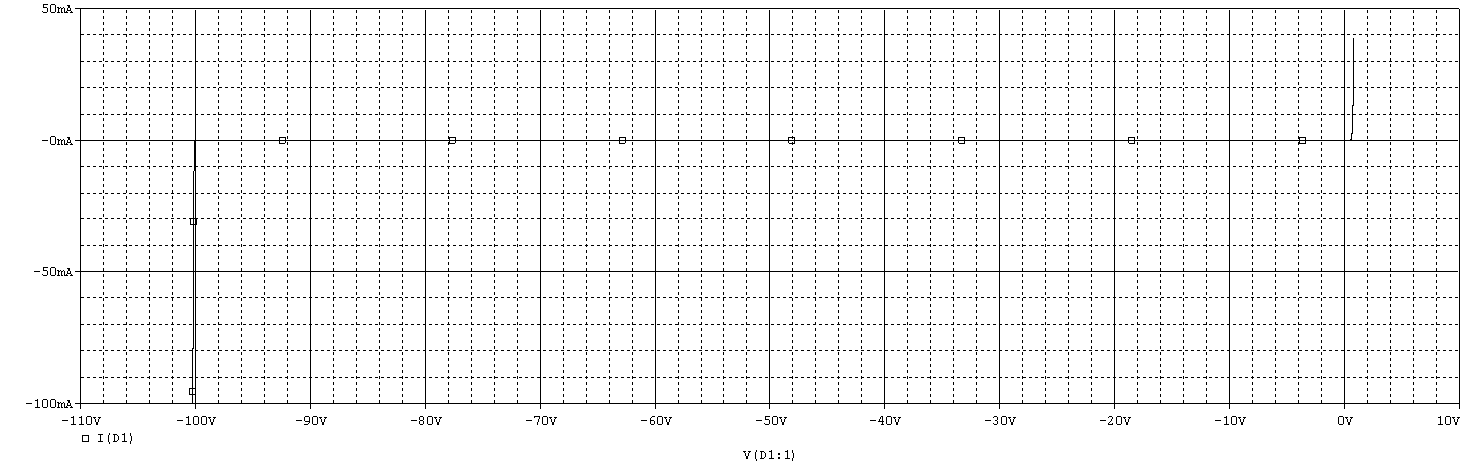
\includegraphics[width=\textwidth]{figure/diode_IV_curve.png}
        \caption{二极管伏安特性曲线图}
        \label{fig:1.3b}
    \end{subfigure}
    \caption{二极管伏安特性曲线设置与结果图示}
    \label{fig:1.3}
\end{figure}

(4)二极管在不同温度下的正向伏安特性曲线

为了得到二极管在不同温度下的正向伏安特性曲线，需要设置直流扫描的次要分析，选择温度作为次要扫描变量，设置温度值为-10℃、0℃、和30℃。
同时曲线坐标轴也需要重新设置，改变X轴范围为0V到1V，Y轴范围为0mA至40mA，如图\ref{fig:1.5}。
\begin{figure}[H]
    \centering
    \begin{subfigure}{0.32\textwidth}
        \centering
        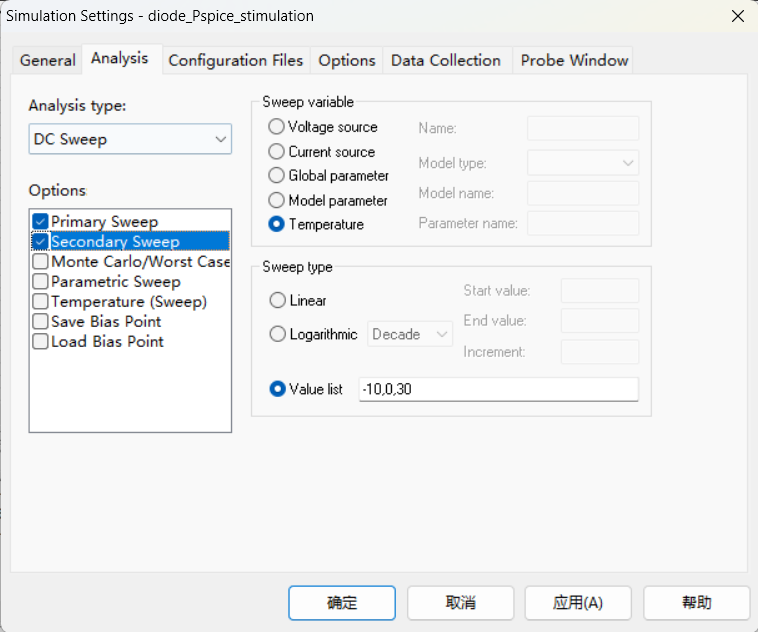
\includegraphics[width=\textwidth]{figure/diode_t_dcsweep_setting.png}
        \caption{直流扫描温度参数设置图}
        \label{fig:1.5a}
   
    \end{subfigure}
    \hfill
    
\begin{subfigure}{0.65\textwidth}
        \centering
        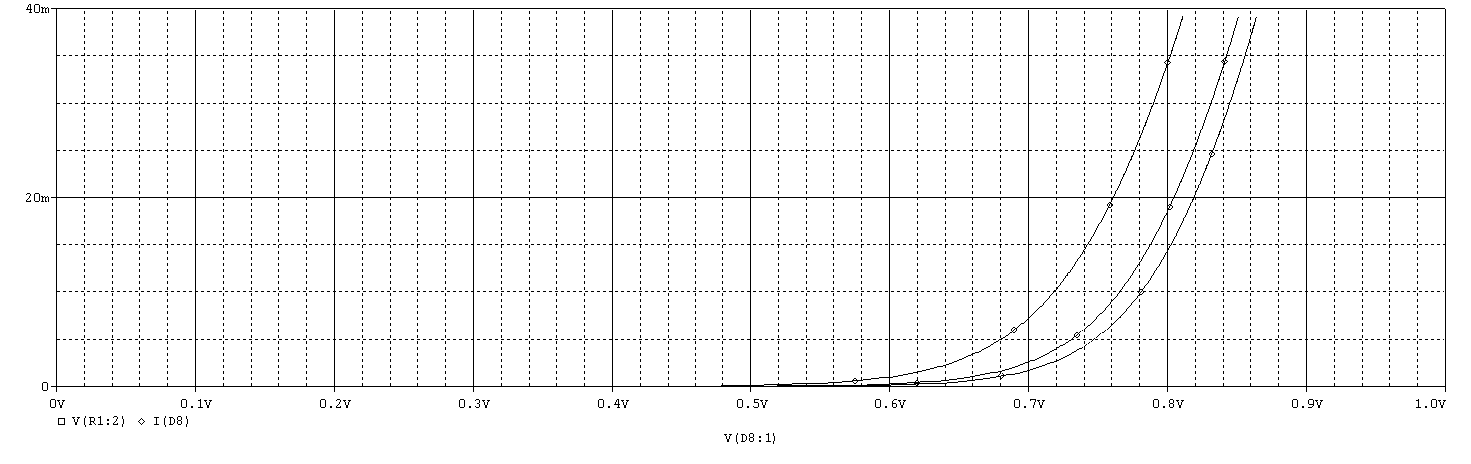
\includegraphics[width=\textwidth]{figure/diode_t_curve.png}
        \caption{二极管在不同温度下正向伏安特性曲线图}
        \label{fig:1.5b}
    \end{subfigure}
    
    \vspace{0.5cm}
    
\begin{subfigure}{0.42\textwidth}
        \centering
        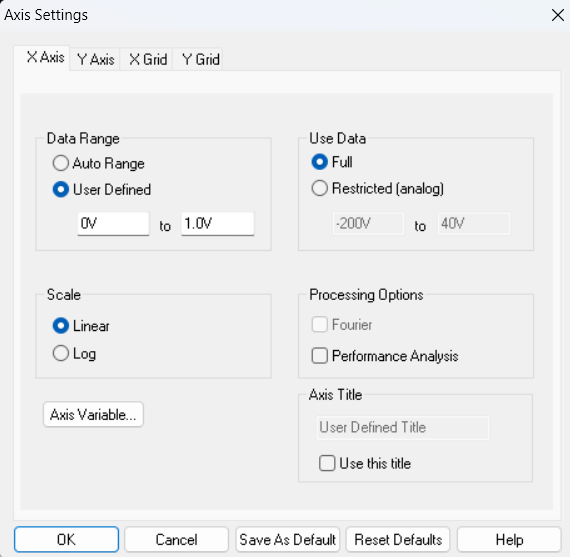
\includegraphics[width=\textwidth]{figure/diode_t_xsetting.png}
        \caption{X轴范围设置图}
        \label{fig:1.5c}
    \end{subfigure}
    \hfill
    
\begin{subfigure}{0.52\textwidth}
        \centering
        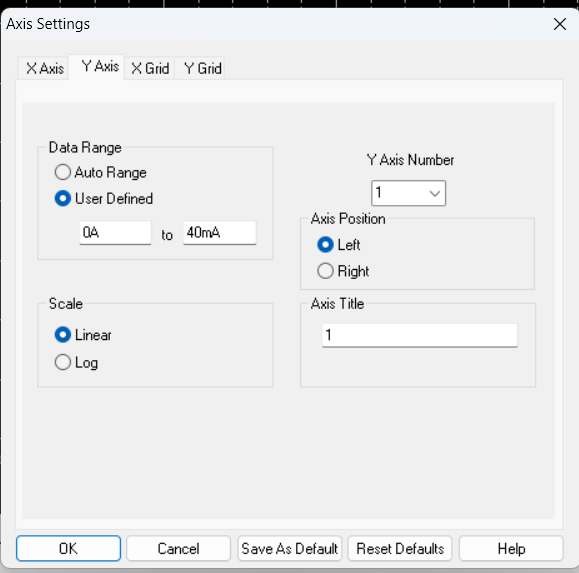
\includegraphics[width=\textwidth,height=0.6\textwidth]{figure/diode_t_ysetting.png}
        \caption{Y轴范围设置图}
        \label{fig:1.5d}
    \end{subfigure}
    \caption{二极管仿真参数设置图示}
    \label{fig:1.5}
\end{figure}

仿真后得到不同温度下二极管的正向伏安特性曲线，如图\ref{fig:1.5b}所示。

从左到右温度依次下降。温度升高时二极管电流增大，温度降低时二极管电流减小。且30°C和0°C时的曲线变化相比于0°C和-10°C时曲线变化更大

(5)二极管两端的电压波形

设置正弦信号源，幅值为10V，频率为1kHz，直流偏置为0V，初始相位为0°，仿真时间为2ms，最大步长为10μs，运行仿真，得到二极管两端的电压波形。
电路图、瞬态扫描参数设置和电压波形如下。

\begin{figure}[H]
    \centering
    \begin{subfigure}{0.31\textwidth}
        \centering
        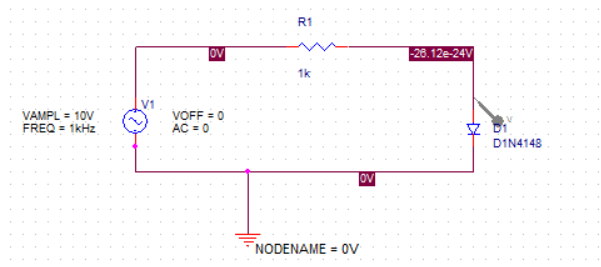
\includegraphics[width=\textwidth]{figure/diode_ac_circuit.png}
        \caption{二极管电压波形测量电路原理图}
        \label{fig:1.6a}
    \end{subfigure}
    \hfill
    
\begin{subfigure}{0.36\textwidth}
        \centering
        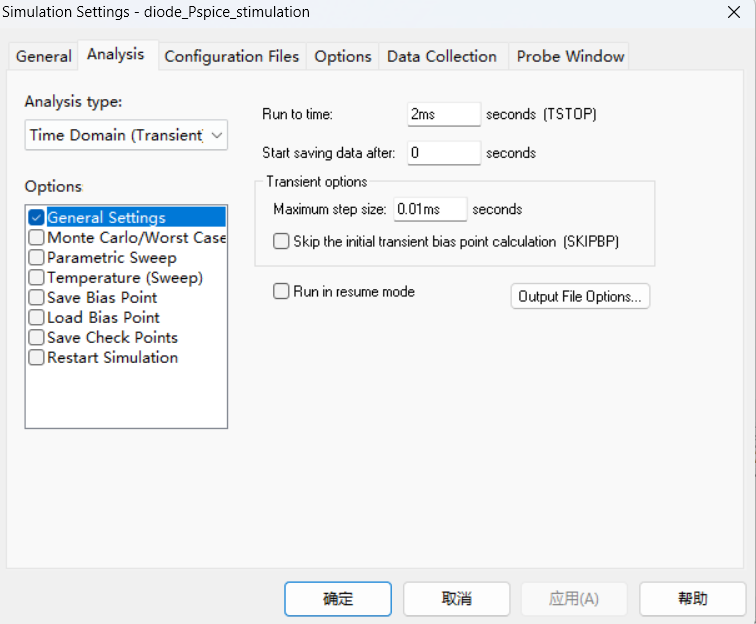
\includegraphics[width=\textwidth]{figure/diode_ac_setting.png}
        \caption{瞬态分析参数设置}
        \label{fig:1.6b}
    \end{subfigure}
    \hfill
    
\begin{subfigure}{0.29\textwidth}
        \centering
        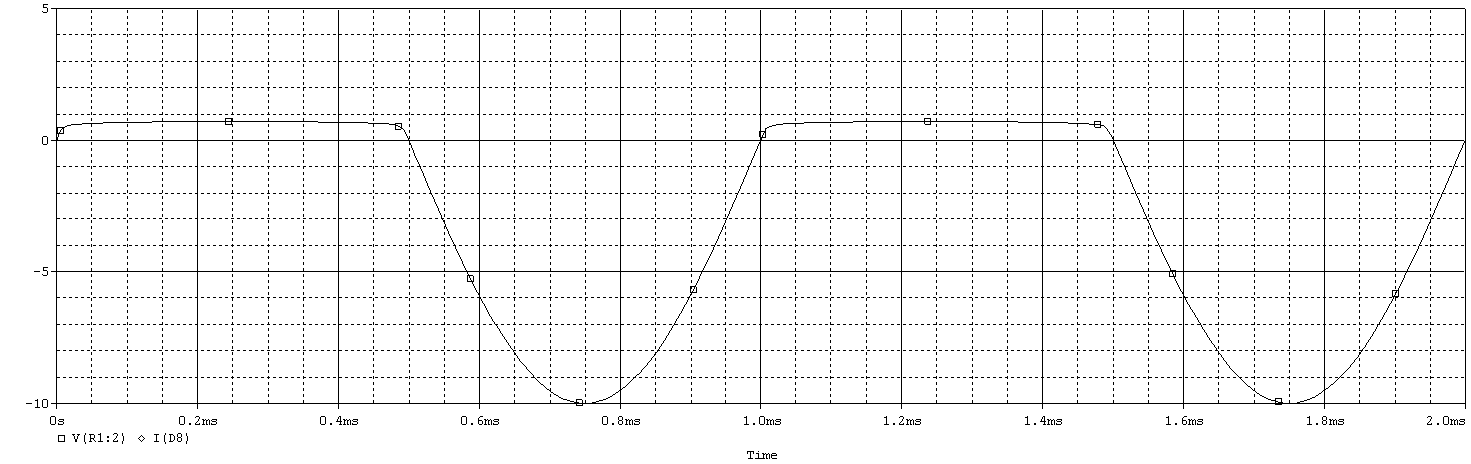
\includegraphics[width=\textwidth]{figure/diode_v_waveform.png}
        \caption{二极管两端电压波形图}
        \label{fig:1.6c}
    \end{subfigure}
    \caption{二极管电压波形仿真}
    \label{fig:1.6}
\end{figure}

\subsection*{3.2 桥式整流电路瞬态分析}
电路组成为正弦信号源VSINC，频率为50Hz，幅值为12V，直流偏置为0V，初始相位为0°；负载电阻R2=1kΩ；四只二极管D1N4148组成桥式整流电路。电路图如图\ref{fig:2.1a}所示。
扫描参数设为：仿真时间为0.04s，最大步长为2ms，如图\ref{fig:2.1b}所示。
使用探针测量输出电压即R2两端的正电位波形，如图\ref{fig:2.1c}所示。

\begin{figure}[H]
    \centering
    \begin{subfigure}{0.35\textwidth}
        \centering
        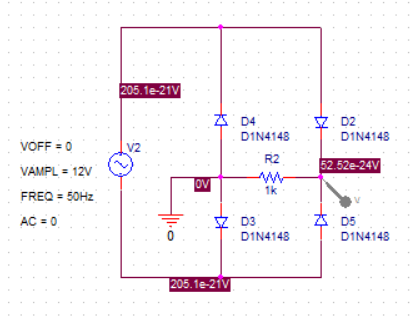
\includegraphics[width=\textwidth]{figure/bridge_circuit.png}
        \caption{桥式整流电路原理图}
        \label{fig:2.1a}
    \end{subfigure}
    \hfill
    
\begin{subfigure}{0.28\textwidth}
        \centering
        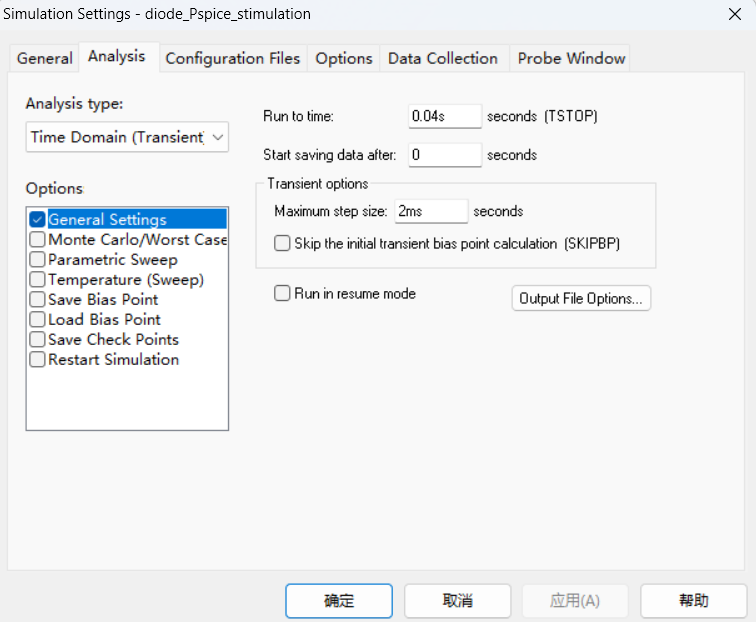
\includegraphics[width=\textwidth]{figure/bridge_setting.png}
        \caption{瞬态分析参数设置}
        \label{fig:2.1b}
    \end{subfigure}
    \hfill
    
\begin{subfigure}{0.33\textwidth}
        \centering
        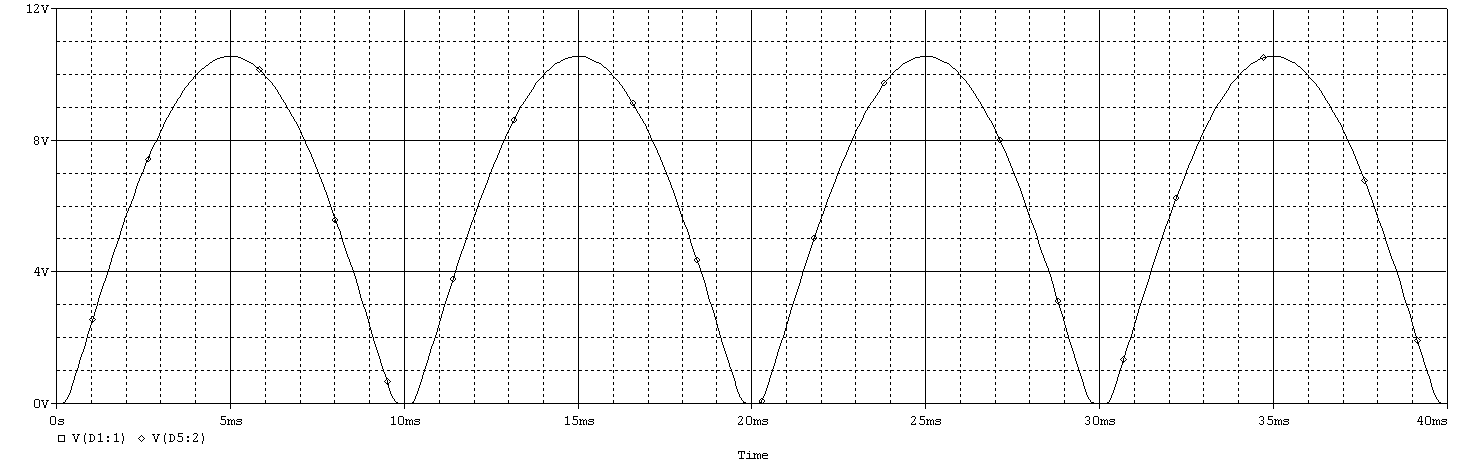
\includegraphics[width=\textwidth]{figure/bridge_waveform.png}
        \caption{输出电压波形图}
        \label{fig:2.1c}
    \end{subfigure}
    \caption{桥式整流电路仿真}
    \label{fig:2.1}
\end{figure}

\subsection*{3.3 稳压二极管电路瞬态分析}
电路组成为正弦信号源VSINC，频率为50Hz，幅值为9V，直流偏置为0V，初始相位为0°；负载电阻R3=5kΩ,R4=10kΩ；两只二极管D1N4148组成稳压二极管电路。电路图如图\ref{fig:2.2a}所示。
扫描参数设为：仿真时间为0.04s，最大步长为2ms，如图\ref{fig:2.2b}所示。
使用探针测量输入电压和输出电压波形，如图\ref{fig:2.2c}所示。

\begin{figure}[H]
    \centering
    \begin{subfigure}{0.38\textwidth}
        \centering
        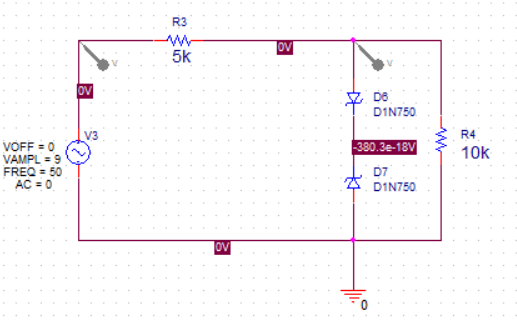
\includegraphics[width=\textwidth]{figure/constant_v_circuit.png}
        \caption{稳压二极管电路原理图}
        \label{fig:2.2a}
    \end{subfigure}
    \hfill
    
\begin{subfigure}{0.27\textwidth}
        \centering
        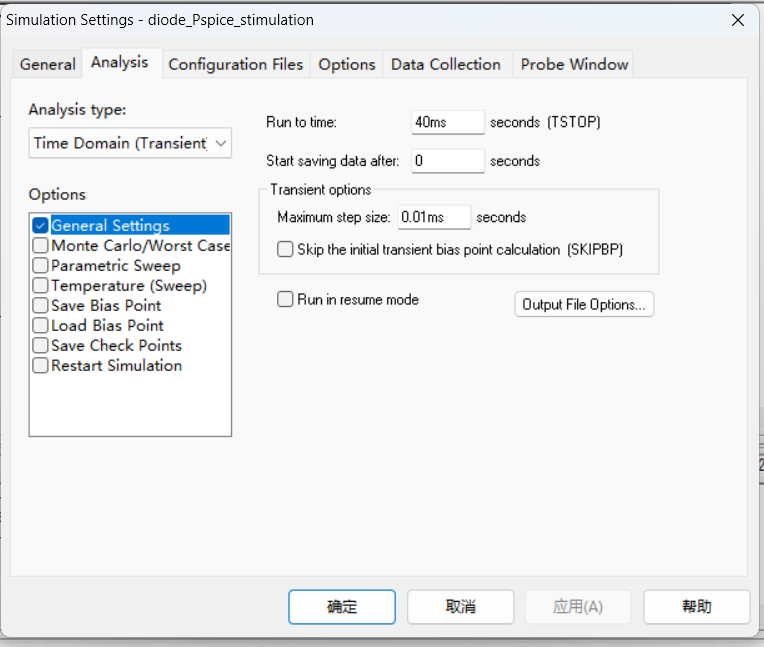
\includegraphics[width=\textwidth]{figure/constant_v_setting.png}
        \caption{瞬态分析参数设置}
        \label{fig:2.2b}
    \end{subfigure}
    \hfill
    
\begin{subfigure}{0.34\textwidth}
        \centering
        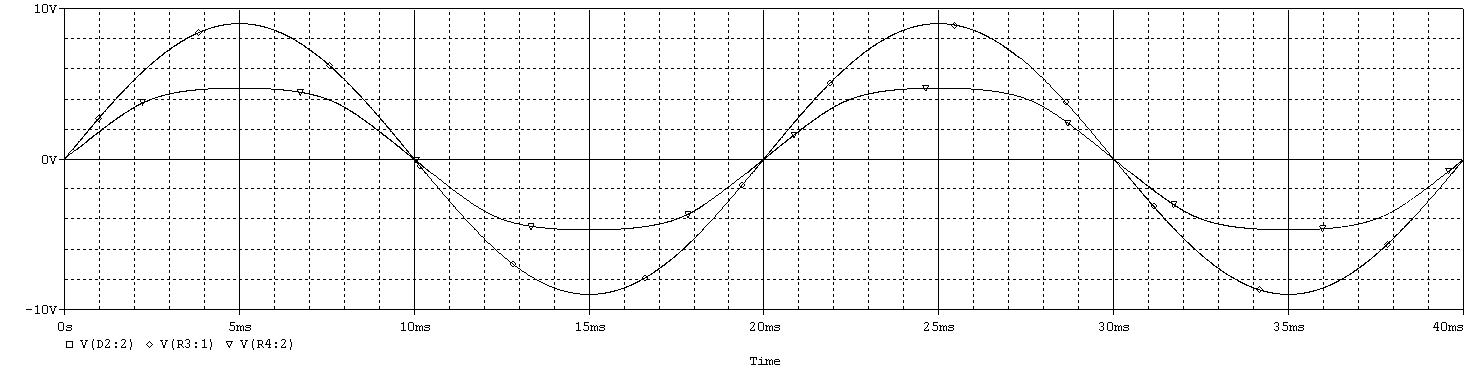
\includegraphics[width=\textwidth]{figure/constant_v_curve.png}
        \caption{输入输出波形对比图}
        \label{fig:2.2c}
    \end{subfigure}
    \caption{稳压二极管电路仿真}
    \label{fig:2.2}
\end{figure}

稳压二极管参数上的稳压值为4.7V，利用measure功能测量波形得到电压值4.73271V，和理论值符合。

\begin{figure}[H]
    \centering
    \begin{subfigure}{0.47\textwidth}
        \centering
        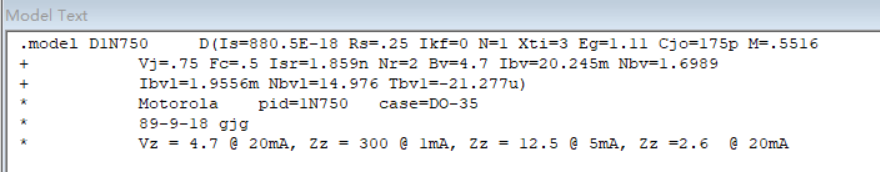
\includegraphics[width=\textwidth]{figure/constant_v_datasheet.png}
        \caption{稳压二极管参数表}
        \label{fig:2.3a}
    \end{subfigure}
    \hfill
    
\begin{subfigure}{0.51\textwidth}
        \centering
        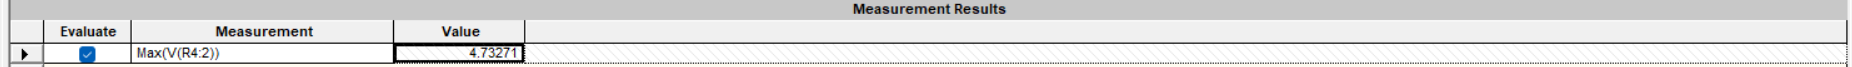
\includegraphics[width=\textwidth]{figure/constant_v_measure.png}
        \caption{测量得到的稳压值4.73271V}
        \label{fig:2.3b}
    \end{subfigure}
    \caption{稳压二极管参数与测量}
    \label{fig:2.3}
\end{figure}

\section*{四、结论}
通过本次实验，我们深入掌握了OrCAD软件的基本使用方法，并成功完成了三类典型电路的仿真分析：

1. 二极管特性仿真方面：获得了完整的二极管伏安特性曲线，观察到其非线性特征——正向导通压降约0.7V，反向截止区漏电流极小，以及反向击穿现象。温度影响研究表明，温度升高会使二极管正向压降略有减小，相同电压下电流增大，体现了PN结的温度敏感性。

2. 桥式整流电路方面：实现了交流到脉动直流的转换，输出波形呈现典型的全波整流特征，峰值接近输入信号的峰值减去两个二极管的正向压降，验证了整流电路的基本工作原理。

3. 稳压二极管电路方面：成功展示了齐纳二极管的稳压功能，当输入电压超过一定阈值后，输出电压稳定在4.73V左右，与器件手册给出的4.7V稳压值基本吻合，误差仅0.69\%，证明了仿真的准确性。

总体而言，OrCAD软件提供了强大的电路设计和仿真能力，能够准确模拟实际器件的电气特性。

\section*{五、心得与体会}
本次OrCAD软件学习实验让我收获颇丰：

首先，我深刻体会到现代EDA工具在电子工程设计中的重要性。相比传统的手工计算和实物搭建，计算机仿真不仅效率更高，还能提供更全面的性能分析，大大缩短了设计周期。特别是温度扫描等高级功能，能够在设计阶段就预见环境因素的影响。

其次，通过实践加深了对半导体器件特性的理解。观察到的二极管实际伏安关系比理想模型复杂得多，这提醒我在后续电路设计中需要考虑更多实际因素。比如在精密应用中，温度补偿可能十分必要。

再者，我认识到软件操作的细节至关重要。如最初未正确设置X轴变量导致无法获得标准的伏安曲线，这体现了精确控制仿真参数的重要性。同样，合理的步长设置对保证波形质量和仿真效率都有显著影响。

最后，本次实验培养了我严谨的科学态度。从电路搭建、参数设置到结果分析，每一步都需要认真对待。特别是在比较实测值与理论值时，学会分析微小差异的来源，这种思维方式对未来从事工程技术工作具有重要意义。

\section*{六、思考题}
1.OrCAD 软件在电路分析及设计过程中起什么作用？

OrCAD软件在现代电路设计中发挥着核心作用：

(1) 提供虚拟实验室环境，可在无实体实体元器件情况下验证设计方案；

(2) 支持多种高级分析（直流、交流、瞬态、噪声、蒙特卡洛等），全面评估电路性能；

(3) 具备强大的参数优化功能，帮助设计师快速找到最优解；

(4) 集成完整的工具链，实现从原理图设计到PCB布局的无缝衔接；

(5) 显著降低成本和时间，避免反复制作样机的资源浪费。

2.用 OrCAD 软件对电路进行仿真分析时，是否要求每个节点必须有标号？在电路中设置节点标号
有何作用？

并非所有节点都必须有标号。接地接地节点、普通连接点可以不专门标注。但是关键节点建议设置标号，其主要作用是：

(1) 便于在Probe中识别和选择特定节点的电压或支路电流；

(2) 在进行某些特定分析（如传输函数分析、噪声分析）时需要指定输入输出节点；

(3) 提高原理图的可读性和维护性；

(4) 在多页设计中实现跨页连接。

3.用 OrCAD 的 PSpice A/D 中的 Probe 图形后处理程序查看图形时，对于不同的分析设置，其缺省
的横坐标是哪个变量？

不同分析的默认横坐标各不相同：

- DC Sweep分析：横坐标为扫描变量本身；

- AC Sweep分析：横坐标为频率；

- Transient分析：横坐标为时间；

- Bias Point分析：无图形输出，只有数值结果。

4.在仿真分析二极管特性测试电路的电压波形时，若瞬态分析不设置 Maximum step size 参数，则
结果会出现什么情况？

若不设置Maximum step size参数可能出现以下问题：

(1) 在信号快速变化的区域（如二极管开关瞬间），自动步长可能导致采样点不足，造成波形失真或丢失重要细节；

(2) 在某些临界状态下可能出现收敛困难，导致仿真失败；

(3) 虽然能加快仿真速度，但牺牲了精度。合理设置此参数能在保证精度的前提下提高效率，特别适用于包含非线性元件的电路仿真。

\end{document}